\documentclass[12pt]{article}
\usepackage[letterpaper, left=0.75in, right=0.75in, top=0.85in, bottom=0.85in, headsep=0.25in, footskip=0.4in]{geometry}
\usepackage[T1]{fontenc}
\usepackage[scaled=0.95]{helvet}
\renewcommand{\familydefault}{\sfdefault}
\usepackage{tikz}
\usetikzlibrary{arrows.meta}
\usepackage{fancyhdr}
\pagestyle{fancy}
\fancyhf{}
\renewcommand{\headrulewidth}{0pt}
\lhead{\small Week NN / Pancake flips / Grades 4--5}
\lfoot{\small Bellingham Math Circle / Week NN / NN-45-v1}
\rfoot{\small \thepage}
\setlength{\parindent}{0pt}
\setlength{\parskip}{6pt}
\definecolor{cakefillc}{RGB}{248,224,170}
\definecolor{cakedrawc}{RGB}{140,95,35}
\definecolor{burntc}{RGB}{85,50,20}
\tikzset{
  cakefill/.style={fill=cakefillc},
  cakedraw/.style={draw=cakedrawc, line width=0.9pt},
  burnt/.style={fill=burntc},
  platedraw/.style={draw=black!55, line width=0.6pt},
  platefill/.style={fill=black!18},
  slot/.style={draw=black!70, dashed, line width=0.8pt},
  spatula/.style={fill=black!65},
  handle/.style={fill=black!40},
  tokdraw/.style={draw=black!70, line width=0.8pt},
  tokfill/.style={fill=black!12},
  breakmark/.style={draw=red!80!black, line width=1.8pt, line cap=round},
}
\newcommand{\problem}[1]{\par\medskip\textbf{Problem #1:}\ }
\begin{document}
A stack is sorted when each pancake sits on a bigger one. To flip, slide the spatula under any pancake and turn that pancake and everything above it over together. Write a stack as its numbers from the top, and a flip as the number of pancakes it turns over.
\par\smallskip\begin{center}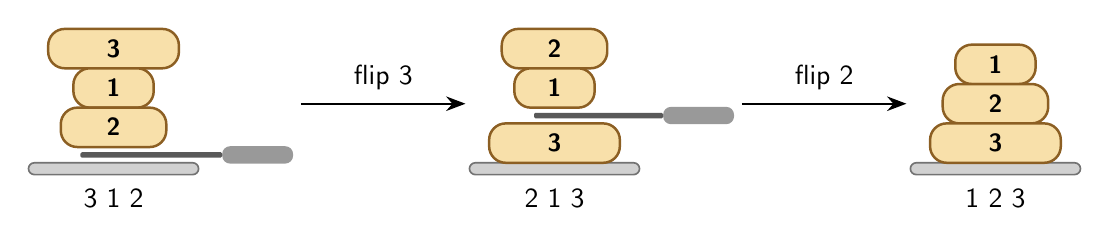
\begin{tikzpicture}
\draw[platedraw, platefill, rounded corners=0.075cm] (-1.080,-0.150) rectangle (1.080,0);
\fill[cakefill] [rounded corners=0.210cm] (-0.830,1.200) rectangle (0.830,1.700);
\draw[cakedraw] [rounded corners=0.210cm] (-0.830,1.200) rectangle (0.830,1.700);
\node[font=\small\bfseries, inner sep=0pt] at (0.000,1.450) {3};
\fill[cakefill] [rounded corners=0.210cm] (-0.510,0.700) rectangle (0.510,1.200);
\draw[cakedraw] [rounded corners=0.210cm] (-0.510,0.700) rectangle (0.510,1.200);
\node[font=\small\bfseries, inner sep=0pt] at (0.000,0.950) {1};
\fill[cakefill] [rounded corners=0.210cm] (-0.670,0.200) rectangle (0.670,0.700);
\draw[cakedraw] [rounded corners=0.210cm] (-0.670,0.200) rectangle (0.670,0.700);
\node[font=\small\bfseries, inner sep=0pt] at (0.000,0.450) {2};
\fill[spatula, rounded corners=0.5pt] (-0.420,0.065) rectangle (1.380,0.135);
\fill[handle, rounded corners=0.099cm] (1.380,-0.010) rectangle (2.280,0.210);
\node[anchor=north, font=\normalsize, inner sep=0pt] at (0.000,-0.330) {3\,\,1\,\,2};
\draw[-{Stealth[length=7pt]}, thick] (2.380,0.750) -- (4.470,0.750);
\node[above, font=\normalsize] at (3.425,0.800) {flip 3};
\draw[platedraw, platefill, rounded corners=0.075cm] (4.520,-0.150) rectangle (6.680,0);
\fill[cakefill] [rounded corners=0.210cm] (4.930,1.200) rectangle (6.270,1.700);
\draw[cakedraw] [rounded corners=0.210cm] (4.930,1.200) rectangle (6.270,1.700);
\node[font=\small\bfseries, inner sep=0pt] at (5.600,1.450) {2};
\fill[cakefill] [rounded corners=0.210cm] (5.090,0.700) rectangle (6.110,1.200);
\draw[cakedraw] [rounded corners=0.210cm] (5.090,0.700) rectangle (6.110,1.200);
\node[font=\small\bfseries, inner sep=0pt] at (5.600,0.950) {1};
\fill[cakefill] [rounded corners=0.210cm] (4.770,0.000) rectangle (6.430,0.500);
\draw[cakedraw] [rounded corners=0.210cm] (4.770,0.000) rectangle (6.430,0.500);
\node[font=\small\bfseries, inner sep=0pt] at (5.600,0.250) {3};
\fill[spatula, rounded corners=0.5pt] (5.340,0.565) rectangle (6.980,0.635);
\fill[handle, rounded corners=0.099cm] (6.980,0.490) rectangle (7.880,0.710);
\node[anchor=north, font=\normalsize, inner sep=0pt] at (5.600,-0.330) {2\,\,1\,\,3};
\draw[-{Stealth[length=7pt]}, thick] (7.980,0.750) -- (10.070,0.750);
\node[above, font=\normalsize] at (9.025,0.800) {flip 2};
\draw[platedraw, platefill, rounded corners=0.075cm] (10.120,-0.150) rectangle (12.280,0);
\fill[cakefill] [rounded corners=0.210cm] (10.690,1.000) rectangle (11.710,1.500);
\draw[cakedraw] [rounded corners=0.210cm] (10.690,1.000) rectangle (11.710,1.500);
\node[font=\small\bfseries, inner sep=0pt] at (11.200,1.250) {1};
\fill[cakefill] [rounded corners=0.210cm] (10.530,0.500) rectangle (11.870,1.000);
\draw[cakedraw] [rounded corners=0.210cm] (10.530,0.500) rectangle (11.870,1.000);
\node[font=\small\bfseries, inner sep=0pt] at (11.200,0.750) {2};
\fill[cakefill] [rounded corners=0.210cm] (10.370,0.000) rectangle (12.030,0.500);
\draw[cakedraw] [rounded corners=0.210cm] (10.370,0.000) rectangle (12.030,0.500);
\node[font=\small\bfseries, inner sep=0pt] at (11.200,0.250) {3};
\node[anchor=north, font=\normalsize, inner sep=0pt] at (11.200,-0.330) {1\,\,2\,\,3};
\end{tikzpicture}\end{center}
\problem{1}Sort each stack with as few flips as you can. Write down your flips.
\par\medskip
\noindent\makebox[\linewidth][s]{\hfill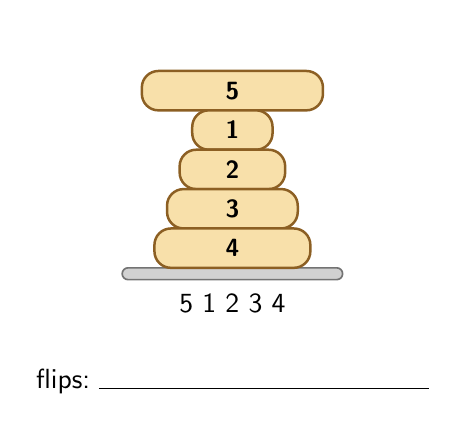
\begin{tikzpicture}
\useasboundingbox (-2.600,-1.880) rectangle (2.600,3.050);
\draw[platedraw, platefill, rounded corners=0.075cm] (-1.400,-0.150) rectangle (1.400,0);
\fill[cakefill] [rounded corners=0.210cm] (-1.150,2.000) rectangle (1.150,2.500);
\draw[cakedraw] [rounded corners=0.210cm] (-1.150,2.000) rectangle (1.150,2.500);
\node[font=\small\bfseries, inner sep=0pt] at (0.000,2.250) {5};
\fill[cakefill] [rounded corners=0.210cm] (-0.510,1.500) rectangle (0.510,2.000);
\draw[cakedraw] [rounded corners=0.210cm] (-0.510,1.500) rectangle (0.510,2.000);
\node[font=\small\bfseries, inner sep=0pt] at (0.000,1.750) {1};
\fill[cakefill] [rounded corners=0.210cm] (-0.670,1.000) rectangle (0.670,1.500);
\draw[cakedraw] [rounded corners=0.210cm] (-0.670,1.000) rectangle (0.670,1.500);
\node[font=\small\bfseries, inner sep=0pt] at (0.000,1.250) {2};
\fill[cakefill] [rounded corners=0.210cm] (-0.830,0.500) rectangle (0.830,1.000);
\draw[cakedraw] [rounded corners=0.210cm] (-0.830,0.500) rectangle (0.830,1.000);
\node[font=\small\bfseries, inner sep=0pt] at (0.000,0.750) {3};
\fill[cakefill] [rounded corners=0.210cm] (-0.990,0.000) rectangle (0.990,0.500);
\draw[cakedraw] [rounded corners=0.210cm] (-0.990,0.000) rectangle (0.990,0.500);
\node[font=\small\bfseries, inner sep=0pt] at (0.000,0.250) {4};
\node[anchor=north, font=\normalsize, inner sep=0pt] at (0.000,-0.330) {5\,\,1\,\,2\,\,3\,\,4};
\node[anchor=base west, font=\normalsize, inner sep=0pt] (fl) at (-2.500,-1.530) {flips:};
\draw[thin] ([xshift=3pt]fl.base east) -- (2.500,-1.530);
\end{tikzpicture}\hfill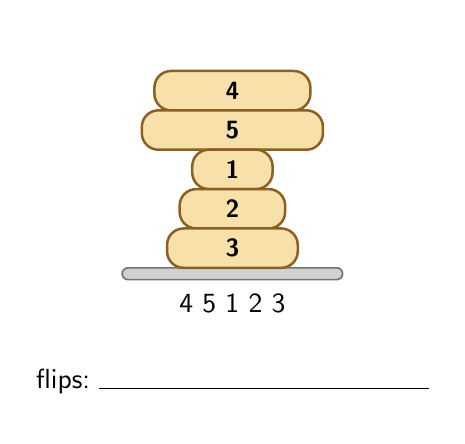
\begin{tikzpicture}
\useasboundingbox (-2.600,-1.880) rectangle (2.600,3.050);
\draw[platedraw, platefill, rounded corners=0.075cm] (-1.400,-0.150) rectangle (1.400,0);
\fill[cakefill] [rounded corners=0.210cm] (-0.990,2.000) rectangle (0.990,2.500);
\draw[cakedraw] [rounded corners=0.210cm] (-0.990,2.000) rectangle (0.990,2.500);
\node[font=\small\bfseries, inner sep=0pt] at (0.000,2.250) {4};
\fill[cakefill] [rounded corners=0.210cm] (-1.150,1.500) rectangle (1.150,2.000);
\draw[cakedraw] [rounded corners=0.210cm] (-1.150,1.500) rectangle (1.150,2.000);
\node[font=\small\bfseries, inner sep=0pt] at (0.000,1.750) {5};
\fill[cakefill] [rounded corners=0.210cm] (-0.510,1.000) rectangle (0.510,1.500);
\draw[cakedraw] [rounded corners=0.210cm] (-0.510,1.000) rectangle (0.510,1.500);
\node[font=\small\bfseries, inner sep=0pt] at (0.000,1.250) {1};
\fill[cakefill] [rounded corners=0.210cm] (-0.670,0.500) rectangle (0.670,1.000);
\draw[cakedraw] [rounded corners=0.210cm] (-0.670,0.500) rectangle (0.670,1.000);
\node[font=\small\bfseries, inner sep=0pt] at (0.000,0.750) {2};
\fill[cakefill] [rounded corners=0.210cm] (-0.830,0.000) rectangle (0.830,0.500);
\draw[cakedraw] [rounded corners=0.210cm] (-0.830,0.000) rectangle (0.830,0.500);
\node[font=\small\bfseries, inner sep=0pt] at (0.000,0.250) {3};
\node[anchor=north, font=\normalsize, inner sep=0pt] at (0.000,-0.330) {4\,\,5\,\,1\,\,2\,\,3};
\node[anchor=base west, font=\normalsize, inner sep=0pt] (fl) at (-2.500,-1.530) {flips:};
\draw[thin] ([xshift=3pt]fl.base east) -- (2.500,-1.530);
\end{tikzpicture}\hfill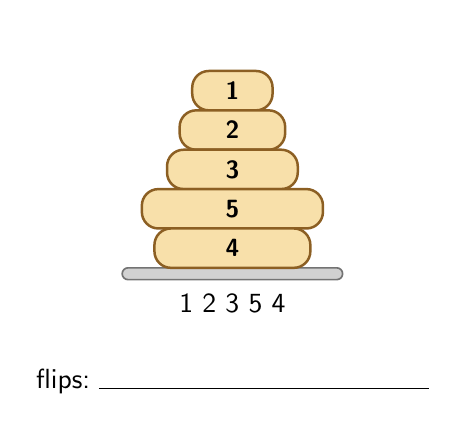
\begin{tikzpicture}
\useasboundingbox (-2.600,-1.880) rectangle (2.600,3.050);
\draw[platedraw, platefill, rounded corners=0.075cm] (-1.400,-0.150) rectangle (1.400,0);
\fill[cakefill] [rounded corners=0.210cm] (-0.510,2.000) rectangle (0.510,2.500);
\draw[cakedraw] [rounded corners=0.210cm] (-0.510,2.000) rectangle (0.510,2.500);
\node[font=\small\bfseries, inner sep=0pt] at (0.000,2.250) {1};
\fill[cakefill] [rounded corners=0.210cm] (-0.670,1.500) rectangle (0.670,2.000);
\draw[cakedraw] [rounded corners=0.210cm] (-0.670,1.500) rectangle (0.670,2.000);
\node[font=\small\bfseries, inner sep=0pt] at (0.000,1.750) {2};
\fill[cakefill] [rounded corners=0.210cm] (-0.830,1.000) rectangle (0.830,1.500);
\draw[cakedraw] [rounded corners=0.210cm] (-0.830,1.000) rectangle (0.830,1.500);
\node[font=\small\bfseries, inner sep=0pt] at (0.000,1.250) {3};
\fill[cakefill] [rounded corners=0.210cm] (-1.150,0.500) rectangle (1.150,1.000);
\draw[cakedraw] [rounded corners=0.210cm] (-1.150,0.500) rectangle (1.150,1.000);
\node[font=\small\bfseries, inner sep=0pt] at (0.000,0.750) {5};
\fill[cakefill] [rounded corners=0.210cm] (-0.990,0.000) rectangle (0.990,0.500);
\draw[cakedraw] [rounded corners=0.210cm] (-0.990,0.000) rectangle (0.990,0.500);
\node[font=\small\bfseries, inner sep=0pt] at (0.000,0.250) {4};
\node[anchor=north, font=\normalsize, inner sep=0pt] at (0.000,-0.330) {1\,\,2\,\,3\,\,5\,\,4};
\node[anchor=base west, font=\normalsize, inner sep=0pt] (fl) at (-2.500,-1.530) {flips:};
\draw[thin] ([xshift=3pt]fl.base east) -- (2.500,-1.530);
\end{tikzpicture}\hfill}

\par\vspace{0.5cm}
\noindent\makebox[\linewidth][s]{\hfill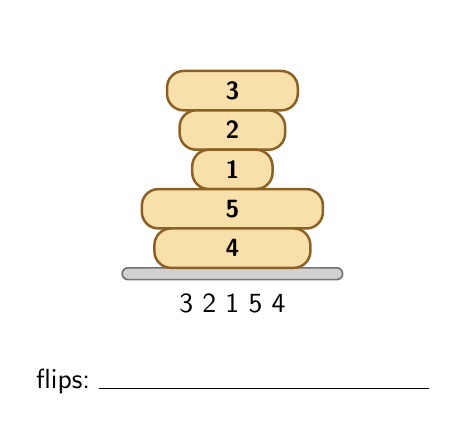
\begin{tikzpicture}
\useasboundingbox (-2.600,-1.880) rectangle (2.600,3.050);
\draw[platedraw, platefill, rounded corners=0.075cm] (-1.400,-0.150) rectangle (1.400,0);
\fill[cakefill] [rounded corners=0.210cm] (-0.830,2.000) rectangle (0.830,2.500);
\draw[cakedraw] [rounded corners=0.210cm] (-0.830,2.000) rectangle (0.830,2.500);
\node[font=\small\bfseries, inner sep=0pt] at (0.000,2.250) {3};
\fill[cakefill] [rounded corners=0.210cm] (-0.670,1.500) rectangle (0.670,2.000);
\draw[cakedraw] [rounded corners=0.210cm] (-0.670,1.500) rectangle (0.670,2.000);
\node[font=\small\bfseries, inner sep=0pt] at (0.000,1.750) {2};
\fill[cakefill] [rounded corners=0.210cm] (-0.510,1.000) rectangle (0.510,1.500);
\draw[cakedraw] [rounded corners=0.210cm] (-0.510,1.000) rectangle (0.510,1.500);
\node[font=\small\bfseries, inner sep=0pt] at (0.000,1.250) {1};
\fill[cakefill] [rounded corners=0.210cm] (-1.150,0.500) rectangle (1.150,1.000);
\draw[cakedraw] [rounded corners=0.210cm] (-1.150,0.500) rectangle (1.150,1.000);
\node[font=\small\bfseries, inner sep=0pt] at (0.000,0.750) {5};
\fill[cakefill] [rounded corners=0.210cm] (-0.990,0.000) rectangle (0.990,0.500);
\draw[cakedraw] [rounded corners=0.210cm] (-0.990,0.000) rectangle (0.990,0.500);
\node[font=\small\bfseries, inner sep=0pt] at (0.000,0.250) {4};
\node[anchor=north, font=\normalsize, inner sep=0pt] at (0.000,-0.330) {3\,\,2\,\,1\,\,5\,\,4};
\node[anchor=base west, font=\normalsize, inner sep=0pt] (fl) at (-2.500,-1.530) {flips:};
\draw[thin] ([xshift=3pt]fl.base east) -- (2.500,-1.530);
\end{tikzpicture}\hfill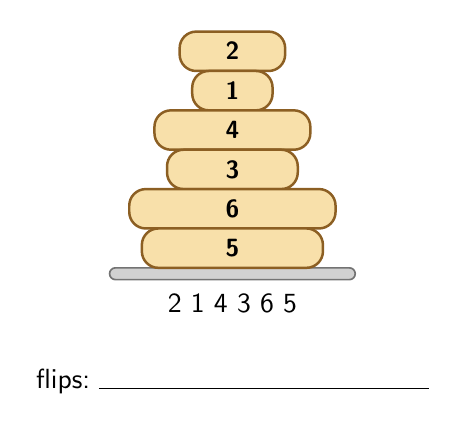
\begin{tikzpicture}
\useasboundingbox (-2.600,-1.880) rectangle (2.600,3.050);
\draw[platedraw, platefill, rounded corners=0.075cm] (-1.560,-0.150) rectangle (1.560,0);
\fill[cakefill] [rounded corners=0.210cm] (-0.670,2.500) rectangle (0.670,3.000);
\draw[cakedraw] [rounded corners=0.210cm] (-0.670,2.500) rectangle (0.670,3.000);
\node[font=\small\bfseries, inner sep=0pt] at (0.000,2.750) {2};
\fill[cakefill] [rounded corners=0.210cm] (-0.510,2.000) rectangle (0.510,2.500);
\draw[cakedraw] [rounded corners=0.210cm] (-0.510,2.000) rectangle (0.510,2.500);
\node[font=\small\bfseries, inner sep=0pt] at (0.000,2.250) {1};
\fill[cakefill] [rounded corners=0.210cm] (-0.990,1.500) rectangle (0.990,2.000);
\draw[cakedraw] [rounded corners=0.210cm] (-0.990,1.500) rectangle (0.990,2.000);
\node[font=\small\bfseries, inner sep=0pt] at (0.000,1.750) {4};
\fill[cakefill] [rounded corners=0.210cm] (-0.830,1.000) rectangle (0.830,1.500);
\draw[cakedraw] [rounded corners=0.210cm] (-0.830,1.000) rectangle (0.830,1.500);
\node[font=\small\bfseries, inner sep=0pt] at (0.000,1.250) {3};
\fill[cakefill] [rounded corners=0.210cm] (-1.310,0.500) rectangle (1.310,1.000);
\draw[cakedraw] [rounded corners=0.210cm] (-1.310,0.500) rectangle (1.310,1.000);
\node[font=\small\bfseries, inner sep=0pt] at (0.000,0.750) {6};
\fill[cakefill] [rounded corners=0.210cm] (-1.150,0.000) rectangle (1.150,0.500);
\draw[cakedraw] [rounded corners=0.210cm] (-1.150,0.000) rectangle (1.150,0.500);
\node[font=\small\bfseries, inner sep=0pt] at (0.000,0.250) {5};
\node[anchor=north, font=\normalsize, inner sep=0pt] at (0.000,-0.330) {2\,\,1\,\,4\,\,3\,\,6\,\,5};
\node[anchor=base west, font=\normalsize, inner sep=0pt] (fl) at (-2.500,-1.530) {flips:};
\draw[thin] ([xshift=3pt]fl.base east) -- (2.500,-1.530);
\end{tikzpicture}\hfill}

\newpage
\problem{2}Find a way to sort any stack of six pancakes, however mixed up it is. What is the most flips your way can need? Explain why it never needs more. How many flips can your way need for a stack of 20 pancakes?
\newpage
\problem{3}Think of each stack as sitting on a plate, and give the plate the number one bigger than the biggest pancake. A break is a place where two touching pancakes, or the bottom pancake and the plate, have numbers that differ by more than 1, such as 1 on 5, or 4 on plate 6 in the stack below.
\par\smallskip\begin{center}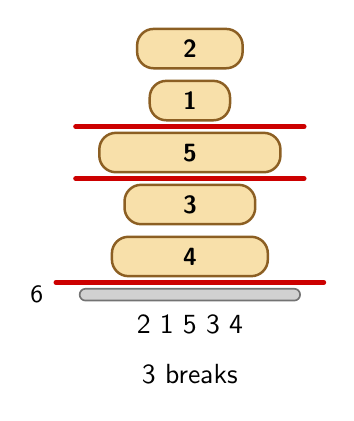
\begin{tikzpicture}
\draw[platedraw, platefill, rounded corners=0.075cm] (-1.400,-0.150) rectangle (1.400,0);
\fill[cakefill] [rounded corners=0.210cm] (-0.670,2.800) rectangle (0.670,3.300);
\draw[cakedraw] [rounded corners=0.210cm] (-0.670,2.800) rectangle (0.670,3.300);
\node[font=\small\bfseries, inner sep=0pt] at (0.000,3.050) {2};
\fill[cakefill] [rounded corners=0.210cm] (-0.510,2.140) rectangle (0.510,2.640);
\draw[cakedraw] [rounded corners=0.210cm] (-0.510,2.140) rectangle (0.510,2.640);
\node[font=\small\bfseries, inner sep=0pt] at (0.000,2.390) {1};
\fill[cakefill] [rounded corners=0.210cm] (-1.150,1.480) rectangle (1.150,1.980);
\draw[cakedraw] [rounded corners=0.210cm] (-1.150,1.480) rectangle (1.150,1.980);
\node[font=\small\bfseries, inner sep=0pt] at (0.000,1.730) {5};
\fill[cakefill] [rounded corners=0.210cm] (-0.830,0.820) rectangle (0.830,1.320);
\draw[cakedraw] [rounded corners=0.210cm] (-0.830,0.820) rectangle (0.830,1.320);
\node[font=\small\bfseries, inner sep=0pt] at (0.000,1.070) {3};
\fill[cakefill] [rounded corners=0.210cm] (-0.990,0.160) rectangle (0.990,0.660);
\draw[cakedraw] [rounded corners=0.210cm] (-0.990,0.160) rectangle (0.990,0.660);
\node[font=\small\bfseries, inner sep=0pt] at (0.000,0.410) {4};
\draw[breakmark] (-1.450,2.060) -- (1.450,2.060);
\draw[breakmark] (-1.450,1.400) -- (1.450,1.400);
\draw[breakmark] (-1.700,0.080) -- (1.700,0.080);
\node[anchor=east, inner sep=1pt, font=\small] at (-1.820,-0.075) {6};
\node[anchor=north, font=\normalsize, inner sep=0pt] at (0.000,-0.330) {2\,\,1\,\,5\,\,3\,\,4};
\node[anchor=north, font=\normalsize] at (0,-0.830) {3 breaks};
\end{tikzpicture}\end{center}
Sort 3 5 2 1 4 with as few flips as you can. It has four breaks. Explain why a stack with four breaks can never be sorted in fewer than four flips.
\par\medskip
\noindent\makebox[\linewidth][s]{\hfill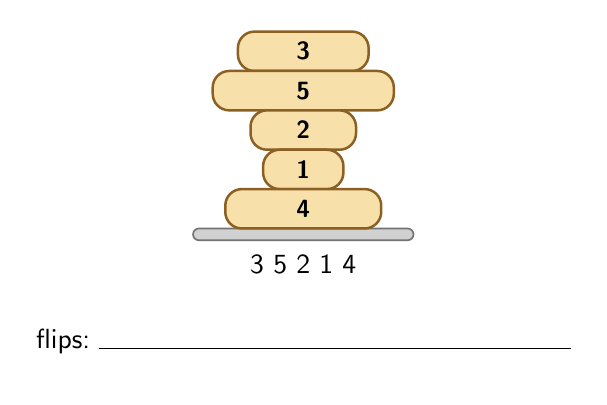
\begin{tikzpicture}
\useasboundingbox (-3.500,-1.880) rectangle (3.500,2.550);
\draw[platedraw, platefill, rounded corners=0.075cm] (-1.400,-0.150) rectangle (1.400,0);
\fill[cakefill] [rounded corners=0.210cm] (-0.830,2.000) rectangle (0.830,2.500);
\draw[cakedraw] [rounded corners=0.210cm] (-0.830,2.000) rectangle (0.830,2.500);
\node[font=\small\bfseries, inner sep=0pt] at (0.000,2.250) {3};
\fill[cakefill] [rounded corners=0.210cm] (-1.150,1.500) rectangle (1.150,2.000);
\draw[cakedraw] [rounded corners=0.210cm] (-1.150,1.500) rectangle (1.150,2.000);
\node[font=\small\bfseries, inner sep=0pt] at (0.000,1.750) {5};
\fill[cakefill] [rounded corners=0.210cm] (-0.670,1.000) rectangle (0.670,1.500);
\draw[cakedraw] [rounded corners=0.210cm] (-0.670,1.000) rectangle (0.670,1.500);
\node[font=\small\bfseries, inner sep=0pt] at (0.000,1.250) {2};
\fill[cakefill] [rounded corners=0.210cm] (-0.510,0.500) rectangle (0.510,1.000);
\draw[cakedraw] [rounded corners=0.210cm] (-0.510,0.500) rectangle (0.510,1.000);
\node[font=\small\bfseries, inner sep=0pt] at (0.000,0.750) {1};
\fill[cakefill] [rounded corners=0.210cm] (-0.990,0.000) rectangle (0.990,0.500);
\draw[cakedraw] [rounded corners=0.210cm] (-0.990,0.000) rectangle (0.990,0.500);
\node[font=\small\bfseries, inner sep=0pt] at (0.000,0.250) {4};
\node[anchor=north, font=\normalsize, inner sep=0pt] at (0.000,-0.330) {3\,\,5\,\,2\,\,1\,\,4};
\node[anchor=base west, font=\normalsize, inner sep=0pt] (fl) at (-3.400,-1.530) {flips:};
\draw[thin] ([xshift=3pt]fl.base east) -- (3.400,-1.530);
\end{tikzpicture}\hfill}

\newpage
\problem{4}Find every stack of pancakes 1, 2, 3 and 4 that cannot be sorted in three flips or fewer. How do you know that each one cannot be sorted in three, and that you have found them all?
\newpage
\problem{5}Find a stack of five pancakes that needs the most flips. Explain why it cannot be sorted in fewer.
\par\vspace{9.5cm}
\problem{6}Stack 4 6 2 5 1 3 has six breaks. Can it be sorted in six flips? If it can, show how. If it cannot, explain why.
\newpage
\problem{7}Now each pancake has a dark side, which must end facing down. Sort each stack with as few flips as you can.
\par\smallskip\begin{center}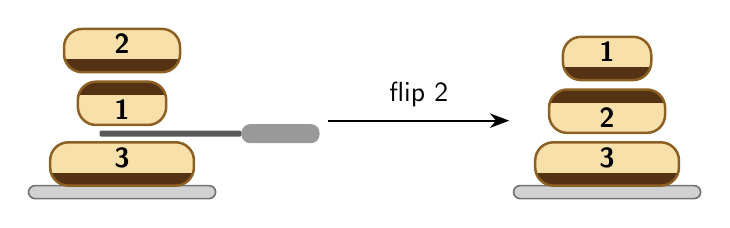
\begin{tikzpicture}
\draw[platedraw, platefill, rounded corners=0.083cm] (-1.188,-0.165) rectangle (1.188,0);
\fill[cakefill] [rounded corners=0.231cm] (-0.737,1.440) rectangle (0.737,1.990);
\begin{scope}
\clip [rounded corners=0.231cm] (-0.737,1.440) rectangle (0.737,1.990);
\fill[burnt] (-0.737,1.440) rectangle (0.737,1.605);
\end{scope}
\draw[cakedraw] [rounded corners=0.231cm] (-0.737,1.440) rectangle (0.737,1.990);
\node[font=\normalsize\bfseries, inner sep=0pt] at (0.000,1.797) {2};
\fill[cakefill] [rounded corners=0.231cm] (-0.561,0.770) rectangle (0.561,1.320);
\begin{scope}
\clip [rounded corners=0.231cm] (-0.561,0.770) rectangle (0.561,1.320);
\fill[burnt] (-0.561,1.155) rectangle (0.561,1.320);
\end{scope}
\draw[cakedraw] [rounded corners=0.231cm] (-0.561,0.770) rectangle (0.561,1.320);
\node[font=\normalsize\bfseries, inner sep=0pt] at (0.000,0.963) {1};
\fill[cakefill] [rounded corners=0.231cm] (-0.913,0.000) rectangle (0.913,0.550);
\begin{scope}
\clip [rounded corners=0.231cm] (-0.913,0.000) rectangle (0.913,0.550);
\fill[burnt] (-0.913,0.000) rectangle (0.913,0.165);
\end{scope}
\draw[cakedraw] [rounded corners=0.231cm] (-0.913,0.000) rectangle (0.913,0.550);
\node[font=\normalsize\bfseries, inner sep=0pt] at (0.000,0.358) {3};
\fill[spatula, rounded corners=0.5pt] (-0.286,0.622) rectangle (1.518,0.699);
\fill[handle, rounded corners=0.109cm] (1.518,0.539) rectangle (2.508,0.781);
\draw[-{Stealth[length=7pt]}, thick] (2.618,0.825) -- (4.917,0.825);
\node[above, font=\normalsize] at (3.768,0.875) {flip 2};
\draw[platedraw, platefill, rounded corners=0.083cm] (4.972,-0.165) rectangle (7.348,0);
\fill[cakefill] [rounded corners=0.231cm] (5.599,1.340) rectangle (6.721,1.890);
\begin{scope}
\clip [rounded corners=0.231cm] (5.599,1.340) rectangle (6.721,1.890);
\fill[burnt] (5.599,1.340) rectangle (6.721,1.505);
\end{scope}
\draw[cakedraw] [rounded corners=0.231cm] (5.599,1.340) rectangle (6.721,1.890);
\node[font=\normalsize\bfseries, inner sep=0pt] at (6.160,1.698) {1};
\fill[cakefill] [rounded corners=0.231cm] (5.423,0.670) rectangle (6.897,1.220);
\begin{scope}
\clip [rounded corners=0.231cm] (5.423,0.670) rectangle (6.897,1.220);
\fill[burnt] (5.423,1.055) rectangle (6.897,1.220);
\end{scope}
\draw[cakedraw] [rounded corners=0.231cm] (5.423,0.670) rectangle (6.897,1.220);
\node[font=\normalsize\bfseries, inner sep=0pt] at (6.160,0.863) {2};
\fill[cakefill] [rounded corners=0.231cm] (5.247,0.000) rectangle (7.073,0.550);
\begin{scope}
\clip [rounded corners=0.231cm] (5.247,0.000) rectangle (7.073,0.550);
\fill[burnt] (5.247,0.000) rectangle (7.073,0.165);
\end{scope}
\draw[cakedraw] [rounded corners=0.231cm] (5.247,0.000) rectangle (7.073,0.550);
\node[font=\normalsize\bfseries, inner sep=0pt] at (6.160,0.358) {3};
\end{tikzpicture}\end{center}
\par\medskip
\noindent\makebox[\linewidth][s]{\hfill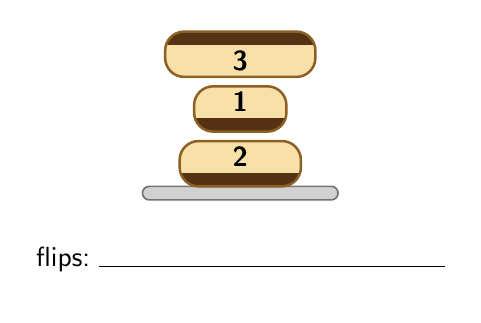
\begin{tikzpicture}
\useasboundingbox (-2.700,-1.373) rectangle (2.700,2.015);
\draw[platedraw, platefill, rounded corners=0.086cm] (-1.242,-0.172) rectangle (1.242,0);
\fill[cakefill] [rounded corners=0.241cm] (-0.954,1.390) rectangle (0.954,1.965);
\begin{scope}
\clip [rounded corners=0.241cm] (-0.954,1.390) rectangle (0.954,1.965);
\fill[burnt] (-0.954,1.792) rectangle (0.954,1.965);
\end{scope}
\draw[cakedraw] [rounded corners=0.241cm] (-0.954,1.390) rectangle (0.954,1.965);
\node[font=\normalsize\bfseries, inner sep=0pt] at (0.000,1.591) {3};
\fill[cakefill] [rounded corners=0.241cm] (-0.586,0.695) rectangle (0.586,1.270);
\begin{scope}
\clip [rounded corners=0.241cm] (-0.586,0.695) rectangle (0.586,1.270);
\fill[burnt] (-0.586,0.695) rectangle (0.586,0.867);
\end{scope}
\draw[cakedraw] [rounded corners=0.241cm] (-0.586,0.695) rectangle (0.586,1.270);
\node[font=\normalsize\bfseries, inner sep=0pt] at (0.000,1.069) {1};
\fill[cakefill] [rounded corners=0.241cm] (-0.770,0.000) rectangle (0.770,0.575);
\begin{scope}
\clip [rounded corners=0.241cm] (-0.770,0.000) rectangle (0.770,0.575);
\fill[burnt] (-0.770,0.000) rectangle (0.770,0.172);
\end{scope}
\draw[cakedraw] [rounded corners=0.241cm] (-0.770,0.000) rectangle (0.770,0.575);
\node[font=\normalsize\bfseries, inner sep=0pt] at (0.000,0.374) {2};
\node[anchor=base west, font=\normalsize, inner sep=0pt] (fl) at (-2.600,-1.022) {flips:};
\draw[thin] ([xshift=3pt]fl.base east) -- (2.600,-1.022);
\end{tikzpicture}\hfill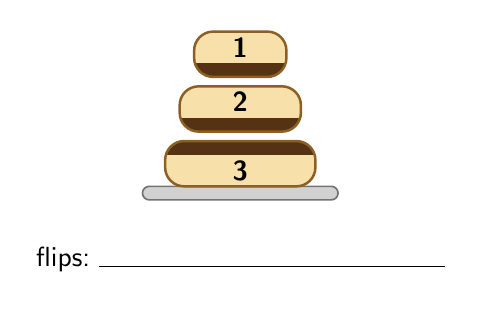
\begin{tikzpicture}
\useasboundingbox (-2.700,-1.373) rectangle (2.700,2.015);
\draw[platedraw, platefill, rounded corners=0.086cm] (-1.242,-0.172) rectangle (1.242,0);
\fill[cakefill] [rounded corners=0.241cm] (-0.586,1.390) rectangle (0.586,1.965);
\begin{scope}
\clip [rounded corners=0.241cm] (-0.586,1.390) rectangle (0.586,1.965);
\fill[burnt] (-0.586,1.390) rectangle (0.586,1.562);
\end{scope}
\draw[cakedraw] [rounded corners=0.241cm] (-0.586,1.390) rectangle (0.586,1.965);
\node[font=\normalsize\bfseries, inner sep=0pt] at (0.000,1.764) {1};
\fill[cakefill] [rounded corners=0.241cm] (-0.770,0.695) rectangle (0.770,1.270);
\begin{scope}
\clip [rounded corners=0.241cm] (-0.770,0.695) rectangle (0.770,1.270);
\fill[burnt] (-0.770,0.695) rectangle (0.770,0.867);
\end{scope}
\draw[cakedraw] [rounded corners=0.241cm] (-0.770,0.695) rectangle (0.770,1.270);
\node[font=\normalsize\bfseries, inner sep=0pt] at (0.000,1.069) {2};
\fill[cakefill] [rounded corners=0.241cm] (-0.954,0.000) rectangle (0.954,0.575);
\begin{scope}
\clip [rounded corners=0.241cm] (-0.954,0.000) rectangle (0.954,0.575);
\fill[burnt] (-0.954,0.402) rectangle (0.954,0.575);
\end{scope}
\draw[cakedraw] [rounded corners=0.241cm] (-0.954,0.000) rectangle (0.954,0.575);
\node[font=\normalsize\bfseries, inner sep=0pt] at (0.000,0.201) {3};
\node[anchor=base west, font=\normalsize, inner sep=0pt] (fl) at (-2.600,-1.022) {flips:};
\draw[thin] ([xshift=3pt]fl.base east) -- (2.600,-1.022);
\end{tikzpicture}\hfill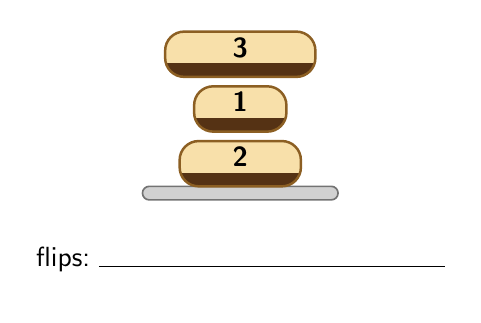
\begin{tikzpicture}
\useasboundingbox (-2.700,-1.373) rectangle (2.700,2.015);
\draw[platedraw, platefill, rounded corners=0.086cm] (-1.242,-0.172) rectangle (1.242,0);
\fill[cakefill] [rounded corners=0.241cm] (-0.954,1.390) rectangle (0.954,1.965);
\begin{scope}
\clip [rounded corners=0.241cm] (-0.954,1.390) rectangle (0.954,1.965);
\fill[burnt] (-0.954,1.390) rectangle (0.954,1.562);
\end{scope}
\draw[cakedraw] [rounded corners=0.241cm] (-0.954,1.390) rectangle (0.954,1.965);
\node[font=\normalsize\bfseries, inner sep=0pt] at (0.000,1.764) {3};
\fill[cakefill] [rounded corners=0.241cm] (-0.586,0.695) rectangle (0.586,1.270);
\begin{scope}
\clip [rounded corners=0.241cm] (-0.586,0.695) rectangle (0.586,1.270);
\fill[burnt] (-0.586,0.695) rectangle (0.586,0.867);
\end{scope}
\draw[cakedraw] [rounded corners=0.241cm] (-0.586,0.695) rectangle (0.586,1.270);
\node[font=\normalsize\bfseries, inner sep=0pt] at (0.000,1.069) {1};
\fill[cakefill] [rounded corners=0.241cm] (-0.770,0.000) rectangle (0.770,0.575);
\begin{scope}
\clip [rounded corners=0.241cm] (-0.770,0.000) rectangle (0.770,0.575);
\fill[burnt] (-0.770,0.000) rectangle (0.770,0.172);
\end{scope}
\draw[cakedraw] [rounded corners=0.241cm] (-0.770,0.000) rectangle (0.770,0.575);
\node[font=\normalsize\bfseries, inner sep=0pt] at (0.000,0.374) {2};
\node[anchor=base west, font=\normalsize, inner sep=0pt] (fl) at (-2.600,-1.022) {flips:};
\draw[thin] ([xshift=3pt]fl.base east) -- (2.600,-1.022);
\end{tikzpicture}\hfill}

\par\vspace{0.5cm}
\noindent\makebox[\linewidth][s]{\hfill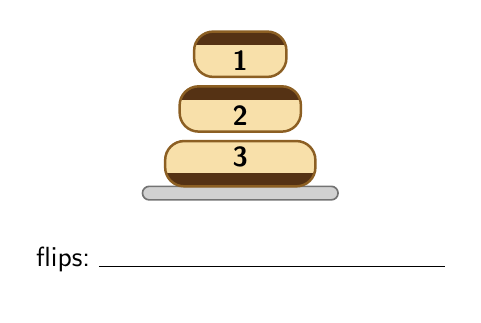
\begin{tikzpicture}
\useasboundingbox (-2.700,-1.373) rectangle (2.700,2.015);
\draw[platedraw, platefill, rounded corners=0.086cm] (-1.242,-0.172) rectangle (1.242,0);
\fill[cakefill] [rounded corners=0.241cm] (-0.586,1.390) rectangle (0.586,1.965);
\begin{scope}
\clip [rounded corners=0.241cm] (-0.586,1.390) rectangle (0.586,1.965);
\fill[burnt] (-0.586,1.792) rectangle (0.586,1.965);
\end{scope}
\draw[cakedraw] [rounded corners=0.241cm] (-0.586,1.390) rectangle (0.586,1.965);
\node[font=\normalsize\bfseries, inner sep=0pt] at (0.000,1.591) {1};
\fill[cakefill] [rounded corners=0.241cm] (-0.770,0.695) rectangle (0.770,1.270);
\begin{scope}
\clip [rounded corners=0.241cm] (-0.770,0.695) rectangle (0.770,1.270);
\fill[burnt] (-0.770,1.098) rectangle (0.770,1.270);
\end{scope}
\draw[cakedraw] [rounded corners=0.241cm] (-0.770,0.695) rectangle (0.770,1.270);
\node[font=\normalsize\bfseries, inner sep=0pt] at (0.000,0.896) {2};
\fill[cakefill] [rounded corners=0.241cm] (-0.954,0.000) rectangle (0.954,0.575);
\begin{scope}
\clip [rounded corners=0.241cm] (-0.954,0.000) rectangle (0.954,0.575);
\fill[burnt] (-0.954,0.000) rectangle (0.954,0.172);
\end{scope}
\draw[cakedraw] [rounded corners=0.241cm] (-0.954,0.000) rectangle (0.954,0.575);
\node[font=\normalsize\bfseries, inner sep=0pt] at (0.000,0.374) {3};
\node[anchor=base west, font=\normalsize, inner sep=0pt] (fl) at (-2.600,-1.022) {flips:};
\draw[thin] ([xshift=3pt]fl.base east) -- (2.600,-1.022);
\end{tikzpicture}\hfill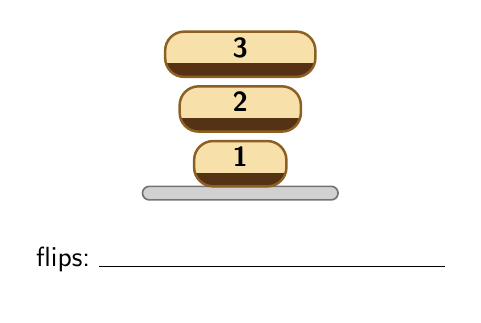
\begin{tikzpicture}
\useasboundingbox (-2.700,-1.373) rectangle (2.700,2.015);
\draw[platedraw, platefill, rounded corners=0.086cm] (-1.242,-0.172) rectangle (1.242,0);
\fill[cakefill] [rounded corners=0.241cm] (-0.954,1.390) rectangle (0.954,1.965);
\begin{scope}
\clip [rounded corners=0.241cm] (-0.954,1.390) rectangle (0.954,1.965);
\fill[burnt] (-0.954,1.390) rectangle (0.954,1.562);
\end{scope}
\draw[cakedraw] [rounded corners=0.241cm] (-0.954,1.390) rectangle (0.954,1.965);
\node[font=\normalsize\bfseries, inner sep=0pt] at (0.000,1.764) {3};
\fill[cakefill] [rounded corners=0.241cm] (-0.770,0.695) rectangle (0.770,1.270);
\begin{scope}
\clip [rounded corners=0.241cm] (-0.770,0.695) rectangle (0.770,1.270);
\fill[burnt] (-0.770,0.695) rectangle (0.770,0.867);
\end{scope}
\draw[cakedraw] [rounded corners=0.241cm] (-0.770,0.695) rectangle (0.770,1.270);
\node[font=\normalsize\bfseries, inner sep=0pt] at (0.000,1.069) {2};
\fill[cakefill] [rounded corners=0.241cm] (-0.586,0.000) rectangle (0.586,0.575);
\begin{scope}
\clip [rounded corners=0.241cm] (-0.586,0.000) rectangle (0.586,0.575);
\fill[burnt] (-0.586,0.000) rectangle (0.586,0.172);
\end{scope}
\draw[cakedraw] [rounded corners=0.241cm] (-0.586,0.000) rectangle (0.586,0.575);
\node[font=\normalsize\bfseries, inner sep=0pt] at (0.000,0.374) {1};
\node[anchor=base west, font=\normalsize, inner sep=0pt] (fl) at (-2.600,-1.022) {flips:};
\draw[thin] ([xshift=3pt]fl.base east) -- (2.600,-1.022);
\end{tikzpicture}\hfill}

\par\vspace{1.0cm}
\problem{8}Find a stack of three pancakes with dark sides that needs the most flips. Draw it with its dark sides.
\par\bigskip
\noindent\makebox[\linewidth][s]{\hfill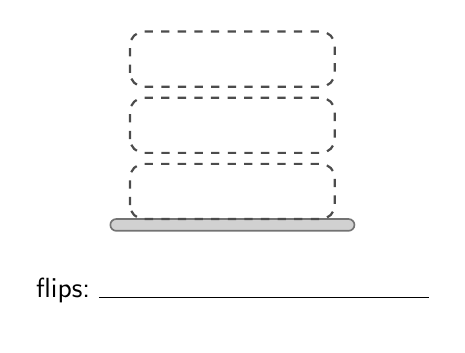
\begin{tikzpicture}
\useasboundingbox (-2.600,-1.350) rectangle (2.600,2.430);
\draw[platedraw, platefill, rounded corners=0.075cm] (-1.550,-0.150) rectangle (1.550,0);
\draw[slot, rounded corners=0.175cm] (-1.300,1.680) rectangle (1.300,2.380);
\draw[slot, rounded corners=0.175cm] (-1.300,0.840) rectangle (1.300,1.540);
\draw[slot, rounded corners=0.175cm] (-1.300,0.000) rectangle (1.300,0.700);
\node[anchor=base west, font=\normalsize, inner sep=0pt] (fl) at (-2.500,-1.000) {flips:};
\draw[thin] ([xshift=3pt]fl.base east) -- (2.500,-1.000);
\end{tikzpicture}\hfill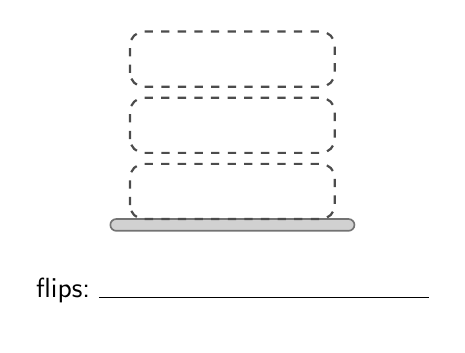
\begin{tikzpicture}
\useasboundingbox (-2.600,-1.350) rectangle (2.600,2.430);
\draw[platedraw, platefill, rounded corners=0.075cm] (-1.550,-0.150) rectangle (1.550,0);
\draw[slot, rounded corners=0.175cm] (-1.300,1.680) rectangle (1.300,2.380);
\draw[slot, rounded corners=0.175cm] (-1.300,0.840) rectangle (1.300,1.540);
\draw[slot, rounded corners=0.175cm] (-1.300,0.000) rectangle (1.300,0.700);
\node[anchor=base west, font=\normalsize, inner sep=0pt] (fl) at (-2.500,-1.000) {flips:};
\draw[thin] ([xshift=3pt]fl.base east) -- (2.500,-1.000);
\end{tikzpicture}\hfill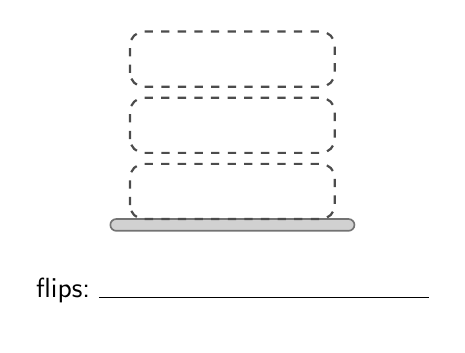
\begin{tikzpicture}
\useasboundingbox (-2.600,-1.350) rectangle (2.600,2.430);
\draw[platedraw, platefill, rounded corners=0.075cm] (-1.550,-0.150) rectangle (1.550,0);
\draw[slot, rounded corners=0.175cm] (-1.300,1.680) rectangle (1.300,2.380);
\draw[slot, rounded corners=0.175cm] (-1.300,0.840) rectangle (1.300,1.540);
\draw[slot, rounded corners=0.175cm] (-1.300,0.000) rectangle (1.300,0.700);
\node[anchor=base west, font=\normalsize, inner sep=0pt] (fl) at (-2.500,-1.000) {flips:};
\draw[thin] ([xshift=3pt]fl.base east) -- (2.500,-1.000);
\end{tikzpicture}\hfill}

\newpage
\problem{9}Find a way to sort any stack of pancakes with dark sides. What is the most flips your way can need for a stack of six?
\end{document}
